\chapter{Generating more flexible locators for System User Interactive Tests}
\section{Introduction}
\label{sec:hpath-introduction}

\subsection{Document Object Model}
\label{sec:hpath-introduction-DOM}

The Document Object Model (DOM) is an application programming interface (API) maintained by the World Wide Web Consortium (W3C) until 2004 and then took over by the Web Hypertext Application Technology Working Group (WHATWG). The goal of the standard is to provide an API allowing to use it with different languages in broad range of environments to generate HTML, RSS and other well-formed XML documents. According to the definition provided by the W3C, the DOM defines the logical structure of documents and the way a document is accessed and manipulated. In this definition, a \emph{document} is the representation of a set of information that may be stored in diverse systems which would traditionally be described as data. In this above definition, XML presents the data as documents and the DOM may be used to manage this data \cite{W3C2004}.

In this work, we view a DOM as a rooted, unranked and ordered tree $D$ where each node $n_D \in N_D$ is labeled. The root node $n_R$ instantiated by a \emph{Document object} allows to associate to each DOM tree $D$ an encoding, a content type, a URL, an origin, a type and a mode. Any node $N_D$ reachable from $n_R$ is said to be contained in the tree and by extension in the document. With different specification, different nodes may have different specialization (\emph{e.g.} providing information about the language of the document, containing raw text, etc.).

\subsection{Hypertext Markup Language}
\label{sec:hpath-introduction-HTML}

Hypertext Markup Language (HTML) is a standard markup derived from the eXtensible Markup Language (XML). It is maintained by the Web Hypertext Application Technology Working Group (WHATWG) and designed to display the Document Object Model (DOM) in a web page. In its current implementation, HTML5, it specifies a set of more granular content models which allow to improve support for multimedia and while maintaining good machine parsing capabilities, ease its readability by humans. The specification of HTML5 can be found in the HTML Living Standard documentation \cite{WHATWG2021}. The HTML syntax consists in a tree differentiating two types of nodes: (1) encoded marker (tags) differentiating bits of information composing the document or defining anchors for multimedia content and referred to as elements $E$ and (2) any other types of nodes containing data\footnote{text node, CDATA section node, comment node,.} or lower level structural properties\footnote{attribute node, processing instruction node, document node, document type node.} of the document $N$.

The root of an HTML document tree is an \emph{html} element, $e_{html}$. The standard enforces the presence of two unique elements as direct children of $e_{html}$ that can appear only once in the document: a \emph{head} element, $e_{head}$ and a \emph{body} element, $e_{body}$. $e_{body}$ is the sectioning root that represents the content of the document. With HTML5 a lot of semantic has been added to children elements of $e_{body}$. In this work we follow the categories presented in the HTML elements reference \cite{MDN2020,WHATWG2021} (Table~\ref{tab:hpath-introduction-html5}).

\begin{table}
\caption{Categories of elements defined by the HTML elements references. When the scope of our category differs from the HTML element references, the original merged categories are mentioned in footnote.}
\label{tab:hpath-introduction-html5}
\begin{center}
\begin{tabular}{>{\raggedright}m{0.4in}>{\raggedright}m{2.6in}}
\toprule
\textbf{\scriptsize{Category}} & \textbf{\scriptsize{Description}}\tabularnewline
\toprule
\scriptsize{\textit{Document Metadata}} & \scriptsize{Elements encapsulating data that are not present in the page, but rather, affects the way content is presented or provides additional information about the document. \emph{e.g.} $E_{link}$, $E_{meta}$ and $E_{style}$.} \tabularnewline
\scriptsize{\textit{Content Sectioning}} & \scriptsize{Elements providing landmark to organize the content of a document into logical pieces. According to the W3C recommendation, the structural information conveyed visually to users should be represented programmatically by the appropriate sectioning element defined by the ARIA landmark roles\cite{W3C2014}. \emph{e.g.} $E_{aside}$, $E_{footer}$, $E_{nav}$, etc.} \tabularnewline
\scriptsize{\textit{Text Content\parnote{\scriptsize{Text Content and Table Content.}}}} & \scriptsize{Elements organizing blocks of content, typically text. \emph{e.g.} $E_{li}$, $E_{p}$, $E_{blockquote}$, etc.} \tabularnewline
\scriptsize{\textit{Inline Text Semantics\parnote{\scriptsize{Inline Text Semantics and Demarcating Edits.}}}} & \scriptsize{Elements formating text such as bold, italic, etc. There are also knowon as \emph{inline} content. \emph{e.g.} $E_{em}$, $E_{strong}$, $E_{cite}$, $E_{small}$, etc.}\tabularnewline
\scriptsize{\textit{Embedded Content\parnote{\scriptsize{Embedded Content, Image \& Multimedia, SVG \& MathML and Web Components.}}}} & \scriptsize{Elements allowing to embedded multimedia resources and other content. They provide information about where to load the content from and how to display it. \emph{e.g.} $E_{img}$, $E_{object}$, $E_{embed}$, $E_{video}$, etc.} \tabularnewline
\scriptsize{\textit{Interactive\parnote{\scriptsize{Interactive and Form.}}}} & \scriptsize{Elements with which a user can interact with. Typically it represents input elements. \emph{e.g.} $E_{input}$, $E_{button}$, etc.} \tabularnewline
\scriptsize{\textit{Scripting}} & \scriptsize{Elements allowing to integrate scripting in order to create dynamic content and Web application. \emph{e.g.} $E_{canvas}$, $E_{noscript}$ and $E_{script}$} \tabularnewline
\bottomrule
\end{tabular}
\end{center}
\parnotes
\end{table}

A specificity of an HTML document is its focus on presentation of the data. Thus, a mechanism to apply styles and positioning to elements under the sectioning root, $e_{body}$, was introduced under the form of the Cascading Style Sheet (CSS). CSS defines a set of styling rules that are to be applied to target elements described by a CSS selector (see Section~\ref{sec:hpath-introduction-css-selector}).

Finally, the HTML standard reserve two elements with no meaning by themselves: the div element, $E_{div}$, from the Content Sectioning category and the span element, $E_{span}$, from the Inline Text Semantics category. These two types do not hold any semantic meaning. Both these elements act as placeholders to mark up user defined semantics common to their children through the use of global attributes, \emph{e.g.} class, id or name. This specific semantics can be useful when used with styling where a subtree can be targeted by a style rule or when interacting with a script to apply some processing to a portion of the document.

\subsection{DOM-based Locators}
\label{sec:hpath-introduction-locators}

A DOM-based locator can be defined as a query language for selecting a subset of targeted nodes $N_{target} \subseteq N_D$ where $N_D$ is the set of nodes contained in the document $D$. Hence, a DOM-based locator is query on a tree $D$ returning a set of nodes $N_{target} \subseteq N_D$ where the size $|N_{target}|$ varies between 0 and $|N_D|$. The HTML standard describes two ways of querying a set of nodes $N_{target} \subseteq N_D$ in a HTML document: XPath and CSS Selector. 

\subsubsection{XPath}
\label{sec:hpath-introduction-xpath}

XML Path Language also known as XPath came from an effort to provide a common syntax and semantics to identify parts of an XML document\cite{W3C2016}. Thus, the query language is not bounded to HTML document but rather to any XML compliant document\footnote{Note that the W3C describes a slightly modified version of the XPath 1.0 standard to interact with HTML documents.}. To query $N_{target}$, XPath relies on the concept of location path. A location path\cite{Gottlob2002} is a series of successive steps traversing the XML tree. At each step, a set of nodes, referred to as context nodes, are uniquely identified. The direct left step of the context node describe the parent node and the right step describes child nodes. During the evaluation of a context node, predicates allow to filter subset of nodes among their siblings (\emph{e.g.} all nodes with a specific attribute). Hence during the location path resolution, the path is traversed from left to right, filtering out part of the tree until it reaches the right-most step and returns the result of the query. If the left-most step is the root of the tree, we call it an absolute XPath (\emph{e.g.} /html/body/div/form/button), otherwise, if the left-most step describes the root of one or many subtrees in the document, it is said to be a relative XPath (\emph{e.g.} //button[@id="validate"]). 

Each step can be defined by a selection node criteria, an optional axis relation and an optional set of predicates\cite{Barton2003}. The selection node criteria defines the element tag from the HTML document. An axis represents a relationship to the context node, and locates relative nodes (parent, self, attributes, preceding, etc.) in the document (\emph{e.g.} //ancestor-or-self::book which selects all ancestors of type book of the context node or the context node itself if it has a tag book). The predicate is an expression contained between brackets after the node criteria allowing more fine grain selection during the evaluation of the step. Predicates can express logical expressions, arithmetic operations or string manipulations \cite{Gottlob2005} (\emph{e.g.} //a[contains(text()="Partial text")]).

\subsubsection{CSS Selector}
\label{sec:hpath-introduction-css-selector}

Contrarily to XPath that relies on location paths, CSS Selector is a structure that determines which elements are matched in the document tree by a pattern described by the locator. Here, the locator is a chain of one or more sequences of simple selectors separated by combinators\cite{W3C2018} represented by ">". The CSS standard defines 6 types of simple selectors supported by the standard: (1) type selector, (2) universal selector, (3) attribute selector, (4) class selector, (5) ID selector and (6) pseudo-class. The type selector qualify an element based on its tag, a class selector based on the class attribute of the element and an ID selector relies on the id attribute of the element. A universal selector is a wild card character (*) allowing to match any substring. The attribute selector is a generalization of the ID selector and the class selector where the name of the attribute and its values are defined. Finally, the pseudo-class concept is introduced to permit selection based on information lying outside the HTML document or that cannot be expressed using other simple selectors (\emph{e.g.} a:visited which allows to target an anchor element, $E_a$, that has already been visited).

Both XPath and CSS Selector rely on internal properties of the elements they target by exploiting the elements attributes (id, class, etc.) which is the cause of their limited flexibility to DOM evolution. In the following section, we present HPath aiming at alleviating this limitation of DOM-based locators.

\section{HPath}
\label{sec:hpath-hpath}

Relying on the HTML standard described in section~\ref{sec:hpath-introduction-HTML}, we proposed \textsc{HTML Path Language (HPath)} a new query language to locate nodes in an HTML document. As its name suggests, our approach is similar to the XPath specification but tailored for HTML documents. While the target is the same as the CSS Selector (both targeting HTML documents), our scope is different. Indeed, our query language aims at providing test automation engineers more expressive and more flexible locators for GUI-based testing. In other words, the goal of our approach is to provide locators that leak as little structural details as possible by relying on properties of the HTML nodes that are rendered on the page to perform the query.

The intuition behind HPath lies in the fact that, if only visible features are permitted in the query, then the resulting locators should be more resilient to iso-functional structural changes. As a consequence, our approach helps to reduce GUI-based test fragility \cite{Thummalapenta2013, Hammoudi2016}. Moreover, relying on rendered properties (such as the label of an input) makes the locator (and, by extension, the test script) easier to understand %by humans reading a test or observing its execution report, because 
as the reliance on structural properties has been minimized.

\begin{table}
\caption{BNF of HPath.}
\label{tab:hpath-hpath-grammar}
\begin{center}
\begin{tabular}{>{\raggedright}m{0.6in}>{\raggedright}m{0.1in} >{\raggedright}m{1.9in}}
\toprule
\code{LocationPath} &\code{:=} &\code{RelLocationPath | '/' RelLocationPath?}\tabularnewline
\code{RelLocationPath} &\code{:=} &\code{'/' Step | RelLocationPath '/' Step}\tabularnewline
\code{Step} &\code{:=} &\code{NameTest Predicate?  | NodeType '(' ')'}\tabularnewline
\code{NameTest} & \code{:=} & \code{Literal}\tabularnewline
\code{Predicate} &\code{:=} &\code{'[' PredicateExpr ']'}\tabularnewline
\code{PredicateExpr} &\code{:=} &\code{Number | FunctionCall}\tabularnewline
\code{FunctionCall} &\code{:=} &\code{FunctionName '(' ')' '=' '"' Literal '"'}\tabularnewline
\code{FunctionName} & \code{:=} & \code{'label' | 'legend' | 'caption' | 'figcaption'}\tabularnewline
\code{NodeType} & \code{:=} & \code{'text'}\tabularnewline
\bottomrule
\end{tabular}
\end{center}
\end{table}

Table~\ref{tab:hpath-hpath-grammar} presents the grammar of HPath in Backus–Naur form (BNF). HPath is expressed as a location path composed of a series of steps (in a XPath fashion, yet using different predicates). Thus, HPath navigates in the HTML documents based on the properties of the nodes it traverses. Each step comprises a \emph{NameTest}, which defines the type (tag) of the context element associated to an optional \emph{Predicate} or a node $N_D \not\in E_D$. Note that only text nodes are supported since they are the only ones being rendered on the page. \emph{Predicate} returns a boolean value filtering out parts of the tree during path traversal. HPath accepts a textual input for the resolution of the predicate (\emph{Literal}) and returns whether or not the value matches the property of the context node. Our implementation is available as a Chrome Plugin\footnote{Available at \emph{link anonymized for double-blind review}} allowing to generate HPath through the browser.

In the remaining of this section we present the properties of HPath empowering it to generate more flexible location paths. We use the notation $E_{\texttt{type}}$ to describe a set of elements of type \texttt{type}, and $e_\texttt{type}$ to refer to a specific element of such a set.

\subsection{Node traversal}
\label{sec:hpath-hpath-node-traversal}

Not all nodes in an HTML document are used for rendering. Indeed, placeholders can be introduced in the DOM to make pages dynamic (animation, dragging, etc.) or to provide better readability for web robots (e.g., Search Engine Optimization). Thus, by definition, these nodes should not appear in the location path when creating flexible locators for GUI-base testing. 

Therefore, the node traversal is done on a rendering tree, generated by the HPath engine, where all elements not affecting the rendering flow are pruned out. Referring to the semantic offered by the HTML standard, two types of elements, $E_{span}$ and $E_{div}$, do not hold any intrinsic semantic by themselves and act as placeholders. Indeed, if no styling is applied to these elements, they are ignored by the rendering engine\cite{Grigorik2019}. Leveraging on this property, HPath ignores any $e_{span}$ or $e_{div}$ that will not affect the rendering flow.  

Since the locator is computed after all styling properties have been assigned to their corresponding elements, all the elements hold all the styling information needed to compute the rendering tree. Then, the algorithm relies on the browser engine for style sheets processing. 

\subsection{Predicates}
\label{sec:hpath-hpath-predicates}

While computing predicates or any other node filtering mechanism, DOM-based locators usually rely heavily on implementation-dependent properties of the elements they visit (\emph{e.g.} id or class). However, these attributes can change without affecting the functionality of a page or any of its visible parts. For example, modifying the id of a button, if not affected by a style rule, will not have any effect on its rendering. Thus, HPath defines a few selected predicates relying on rendered properties. During the predicate resolution, if the extracted text matches the value provided, it returns a true value, false otherwise. The predicates can take the following form:

\begin{itemize}
    \item \textbf{label} Most of the interactive elements $E_{interactive}$ can be associated with a label element, $E_{label}$ to provide a textual clue about their functionality (\emph{e.g.} Label "Name" associated to a textual input so the users know they have to type their name). The HTML standard defines two strategies to link those elements: (1) $e_{label}$ is a direct parent of $e_{interactive}$ or (2) $e_{label}$ is a sibling of $e_{interactive}$ where the value of the attribute \emph{for} of $e_{label}$ equals the value of the attribute \emph{id} of $e_{input}$. The \textbf{label} predicate extracts the textual content (see Section~\ref{sec:hpath-hpath-text-extraction}) of $e_{label}$ associated with the context $e_{interactive}$. 
    
    \item \textbf{legend} Related children elements of a form element ($E_{form}$) can be grouped together through the use of fieldset element ($E_{fieldset}$). Any $e_{fieldset} \in E_{fieldset}$ can be associated with a textual value defined in a legend element, $e_{legend}$. According to the standard, if $e_{legend}$ is a direct child of $e_{fieldset}$, then it is associated to the parent $e_{fieldset}$. The \textbf{legend} predicate extracts the textual content of a $e_{legend}$ associated to the context $e_{fieldset}$. 
    
    \item \textbf{caption} Table elements, $E_{table}$, can be assigned a caption through the use of a caption element $E_{caption}$. According to the standard, if a $e_{caption}$ is a direct child of a $e_{table}$, then it is associated to the parent $e_{table}$. The \textbf{caption} predicate extracts the textual content of a $e_{caption}$ associated to the context $e_{table}$. 
    
    \item \textbf{figcaption} Figure elements, $E_{figure}$, can be assigned a caption through the use of a caption element $E_{figcaption}$. According to the standard, if $e_{figcaption}$ is a direct child of $e_{figure}$, then it is associated to the parent $e_{figure}$. The \textbf{figcaption} predicate extracts the textual content of $e_{figcaption}$ associated to the context $E_{figure}$. 
\end{itemize}

If no predicate can be generated to compute the location path, then the resulting path resembles the one that would be generated by the XPath algorithm, i.e., with only positioning predicate and no axis. The difference, however, is that HPath does not compute the path on the actual DOM but on the rendering tree (as described in Section~\ref{sec:hpath-hpath-node-traversal}).

\subsection{Content Extraction}
\label{sec:hpath-hpath-text-extraction}

In the current implementation of HPath, all predicates (except the positioning predicate) rely on textual information visible on the page. To extract the content of a text under an element, XPath simply extracts the content of the text node, $n_{text}$, which is a direct child of the context element. HPath goes beyond this procedure and analyzes styling information contained in the elements from the Inline Text Semantics category (see Table~\ref{tab:hpath-introduction-html5}). HPath takes advantages of this semantic and filters out any element from this category when extracting text. The resulting $n_{text}$ are then merged together to reconstruct the text that will be used by the predicates for evaluation. For example the "<b>Hello</b> world" is transformed to "Hello world".

\section{Research Questions}
\label{sec:hpath-rqs}

HPath makes a strong assumption on the type of web elements it can successfully locate and properly describe. Hence, to enable the evaluation of its capability, we investigate first which web elements are predominantly targeted by GUI-based tests. Thus, we ask:

\begin{description} 
\item[\textbf{RQ1}:]
\emph{Which categories of elements are predominantly targeted by GUI-based test scripts?} 
\end{description} 

Next, we evaluate our new approach, HPath, and compare its performances in terms of properties of web elements it can leverage. We compare it against two algorithms generating XPath, namely, \emph{absolute XPath} and \emph{Robula+}. This leads to the following research question:

\begin{description} 
\item[\textbf{RQ2}:]
\emph{Which element properties are exploited by the different location path strategies?} 
\end{description} 
        
Finally, we investigate the resilience against SUT evolution of HPath and compare it to the two XPath generation algorithms used in RQ2 and express the final research question as follow:

\begin{description} 
\item[\textbf{RQ3}:]
\emph{What is the resilience against SUT evolution of the different strategies?} 
\end{description} 

\section{Research Protocol}
\label{sec:hpath-protocol}

This section presents the experimental setup for the case studies to answer our research questions. The goal of this study is to analyze the impact of using different second-generation locators in web testing. To qualify the performances of a strategy we rely on two main concepts: the properties of an element it can leverage to select it and its resilience to changes happening during the SUT evolution. In this study, the properties are measured by the length of the location path and the presence of predicates in any step of the location path. The resilience to change of a locator is evaluated by its propensity to not being able to locate an element following a change in the HTML document.

\subsection{Projects Collection}
\label{sec:hpath-protocol-projects}

To select adequate projects for a case study, we mine repositories from Github, using its search API which allows to apply queries to filter the result from the Github database. Because of the restrictions of the mining process described in Section~\ref{sec:hpath-protocol-elements}, we have to isolate projects with tests written in Java and exercising the Selenium API. Furthermore, both application code and test code need to be versioned in the same repository in order to be able to go back in time and run test suites for previous versions.

Because of the dynamic nature of our analysis, we need to be able to compile the projects and run them on successive versions. Despite our best effort, most of the projects we gathered could not be executed in our experimental setup (missing dependencies, outdated build tools). Thus, this process yielded 2 large web based open-source systems: OpenOLAT\footnote{https://github.com/OpenOLAT/OpenOLAT}, a web-based e-learning platform and MISO LIMS\footnote{https://github.com/miso-lims/miso-lims}, a lab information management system designed for tracking next-generation sequencing experiments. Both projects rely on a Java backend that is communicating with a relational database management system. For the front end, both use HTML, CSS and Javascript however MISO LIMS is relying on the HTML4 standard while OpenOLAT is using the HTML5 standard. Finally, both project adopt a multi-tier architecture relying on different services working in concert.

\begin{table}
\caption{Web Applications used in our experiments. Column \emph{\#Releases} presents the number of releases collected, \emph{KLOC} is the number of lines of code in the last release, \emph{\#Tests} is the rounded average number of integration tests per release and \emph{\#Locators} is the total number of locators recorded.}
\label{tab:hpath-protocol-projects}
\begin{center}
\begin{tabular}{>{\raggedright}m{0.4in}>{\raggedleft}m{0.4in}>{\raggedleft}m{0.4in}>{\raggedleft}m{0.4in}>{\raggedleft}m{0.4in}}
\toprule
\textbf{\scriptsize{Project}} & \textbf{\scriptsize{\#Releases}} & \textbf{\scriptsize{KLOC}} & \textbf{\scriptsize{\#Tests}} & \textbf{\scriptsize{\#Locators}} \tabularnewline
\toprule
\scriptsize{\textit{OpenOLAT}} & \scriptsize{8} & \scriptsize{1308} & \scriptsize{154} & \scriptsize{216424} \tabularnewline
\scriptsize{\textit{MISO LIMS}} & \scriptsize{57} & \scriptsize{326} & \scriptsize{8} & \scriptsize{15672} \tabularnewline
\bottomrule
\end{tabular}
\end{center}
\end{table}

Table~\ref{tab:hpath-protocol-projects} presents some key metrics of the projects under study. The 57 version of MISO LIMS were collected between March 2019 and November 2020 and the 8 versions of OpenOLAT span from November 2018 to August 2020. 

The low number of versions for the OpenOLAT project (8 versions) is due to the fact that earlier versions could not be compiled (Maven Plugin not supported). While both projects are quite large in terms of lines of code, we can see that the developers of the project MISO LIMS do not rely heavily on GUI-based testing, with an average number of 8 tests per version.

\begin{figure}
\centering
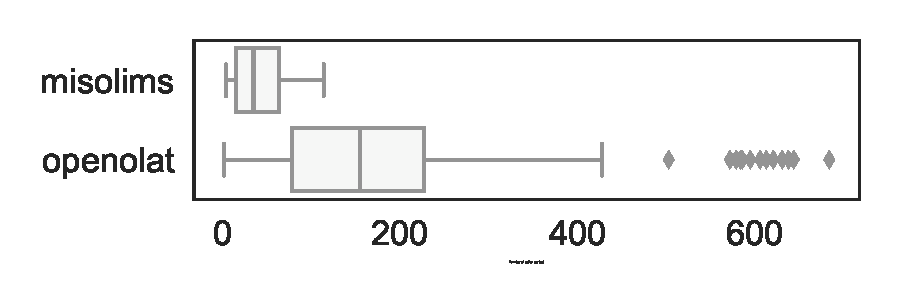
\includegraphics[width=0.8\columnwidth]{figures/locators/selector-per-test-dist.pdf}
\caption{Number of actions triggered by test.}  
\label{fig:hpath-protocol-actions}
\end{figure}

Figure~\ref{fig:hpath-protocol-actions} presents the number of actions triggered by the tests for each project under study. In average, the number of actions triggered by a test is 170 for the OpenOLAT project and about 42 for the MISO LIMS project. One intriguing point shown by the figure is the presence of tests not containing any interaction with the application through Selenium. These are tests not targeting the SUT through the user interface but rather directly interacting with the API of the application or the RDBMS itself.

\subsection{Mining Target Elements}
\label{sec:hpath-protocol-elements}

We developed a tool called \mercator\footnote{Available at \textit{link not available for double blind process}} to capture the state of the pages and the DOM-based locators used to interact with it in the test suites. More specifically, \mercator\ instruments method calls \emph{findElement} and \emph{findElements} from the class \emph{RemoteWebDriver} offered by the Selenium API. Hence, at runtime, \mercator\ captures the following data every time a test exercises a DOM-based locator: (1) information about the state of the current web page \emph{i.e.} complete dump of the DOM, size of the window and current URL; (2) information about the test \emph{i.e.} test name, call stack, inference on the previous call stack; (3) information about the locator \emph{i.e.} locator strategy, locator value; (4) information about the project \emph{i.e.} repository URL, commit id, previous commit id, commit date. This process is repeated for each version defined in the configuration of \mercator. For this study, we select every release of the projects. We restrict our study to releases because the projects rely on external dependencies which are not stable during the development cycle, thus, leading to code that cannot compile due to missing dependencies (SNAPSHOT). Furthermore, using releases increases the chances of observing evolution between two versions, thus, avoiding meaningless computation.

The most sensitive aspect of this process is collecting the DOM dumps. Indeed, as explained in Section~\ref{sec:hpath-introduction-HTML}, a HTML document can contain links to other resources such as multimedia and CSS style sheet stored externally. Thus, in order for the dump to be usable as a single HTML document file, during the instrumentation, a complete HTML document with no external dependencies needs to be computed. This is done by inlining all the CSS style sheets in the header, and providing placeholders for all multimedia content retaining their attributes, size and position. Furthermore, all properties computed by JavaScript are inlined in the style attribute of the elements and all script elements are removed from the dump. This is possible because pages are captured after the execution of any JavaScript routine altering the structure of the DOM tree. Finally, comment nodes and any formatting of the HTML document not affecting its content (line returns between to subsequent elements) are removed in order to limit syntactic differences between dumps.

This process requires a non negligible amount of time (between 200ms to up to 1500ms during our experiments) depending on the complexity of the page. This delay causing tests to run slower breaks some of the test that are bounded by a maximum allocated time budget (\emph{timeout}). This leads us to use a strategy to monitor changes in the DOM tree to minimize the number of time the state has to be computed. Unfortunately, this changes failed to detect changes not altering the tree but modifying external properties of the elements (mostly hovering and selections in table) which lead to generating locators in our dataset that are not valid, 20.09\% for MISO LIMS and 8.57\% for OpenOLAT. We deem this tradeoff reasonable compared to the alternative where observe about 35\% of the tests failing due to our instrumentation.

One of the goals of the study being to investigate the resilience to SUT evolution of the DOM-based locators, it is mandatory to devise a strategy to compute the lineage of a locator across versions. To achieve this objective, we rely on the change log computed by the versioning system Git. \mercator\ enriches the data it records (locator and DOM) with information about the version and the test that is currently running. Then using the current stack trace and the change log between the current version and the previous version (identified by their commit IDs) it is able to offer an approximation of the stack trace in the previous commit. To do so, we use an algorithm that will recompute the stack trace in the previous version, taking into account line additions and deletions in the test code. This process is described in details in Section~\ref{sec:hpath-protocol-pairs}.

Finally, the last step of this process is the extraction of the elements themselves. Each data point generated by \mercator\ contains a locator and its associated HTML document. Thus, by querying the DOM with the collected locators, we can retrieve the elements targeted by the tests.

\subsection{RQ1: Target Elements}
\label{sec:hpath-protocol-rq1}

% The Selenium API offers different strategies to locate web elements as shown in Table~\ref{tab:selenium_strategies}. 

% \begin{table}[!t]
% \def\arraystretch{1.0}
% \caption{Element selection strategies defined by the Selenium API.}
% \label{tab:selenium_strategies}
% \begin{center}
% \begin{tabular}{>{\raggedright}m{0.5in}>{\raggedright}m{2.5in}}
% \toprule
% \textbf{\scriptsize{Strategy}} & \textbf{\scriptsize{Description}}\tabularnewline
% \toprule
% \scriptsize{\textit{class name}} & \scriptsize{Locates elements whose class attribute contains the search value.} \tabularnewline
% \scriptsize{\textit{css selector}} & \scriptsize{Locates elements matching the CSS selector.} \tabularnewline
% \scriptsize{\textit{id}} & \scriptsize{Locate elements whose id attribute matches the search value.} \tabularnewline
% \scriptsize{\textit{link text}} & \scriptsize{Locates anchor elements, $E_a$, whose inner text matches the search value.} \tabularnewline
% \scriptsize{\textit{patial link text}} & \scriptsize{Locates anchor elements, $E_a$, whose inner text contains the search value.} \tabularnewline
% \scriptsize{\textit{tag name}} & \scriptsize{Locates elements whose tag name matches the search value.} \tabularnewline
% \scriptsize{\textit{xpath}} & \scriptsize{Locates elements matching the location path.} \tabularnewline
% \bottomrule
% \end{tabular}
% \end{center}
% \end{table}

The approach that we propose, HPath, makes the assumption that the interactions with the HTML document mainly targets visible elements, \emph{i.e.} elements rendered on the web page. 
%As explained in Section~\ref{sec:Introduction}, each test step is a triple composed of an action to be performed, an element targeted by a locator and potentially a value to pass to the element (\emph{e.g.} some text to fill a field in form).

The assumption that we make is that a test should interact with elements to navigate through the states of the web application then make assertions on visible elements to validate the proper execution of the test as a human would. Thus, not all elements of the HTML document hold the same value for the testers. To assess this hypothesis and answer RQ1, we extract the type (tags) of the elements targeted by the tests. Comparing this distribution with the one contained in the HTML document, we can assess which element types tests typically interact with. 

Furthermore, providing empirical evidence on which type of elements tests typically interact with can help researchers. Indeed, in previous work, when a GUI-based test suite is not available, some studies targeted elements systematically\cite{Cohen2015, Leotta2015, Aldalur2017, Eladawy2018} while other generated test scripts\cite{Grechanik2009, Montoto2011, Kirinuki2019}. Unfortunately, studies relying on \emph{in vivo} GUI-based test suites are usually conducted on industrial projects and the source code is not available\cite{Thummalapenta2013, Yandrapally2014}. While there exists studies tackling the question of the evolution and the characteristics of GUI-based tests \cite{Christophe2014, Rwemalika2019}, they usually rely on static analysis and do not convey information about locators and their target elements. Thus, understanding which type of elements are targeted by testers would allow researchers to create benchmarks to evaluate their approaches by following the same distributions observed in other projects when no tests are available.

\subsection{RQ2: Element Properties Used by Locators}
\label{sec:hpath-protocol-rq2}

In order to evaluate our approach, we compare it against two approaches to generate XPath: absolute XPath and Robula+. We select XPath algorithms because our approach is a derivative of XPath with the aim of addressing one of its limitation: its reliance on structural properties of the HTML document, making HPath more flexible to changes of the internal document structure.

The first algorithm, absolute XPath, builds an XPath where each step can only rely on a positional predicate. Thus, it does not rely on any attributes such as id, class or name and can be seen as the most naive form of XPath generation. Note that when using the absolute XPath algorithm, the deeper an element is nested in a DOM tree, the longer the location path. Thus, this algorithm tends to leak the overall structure of the DOM, where any change in the node hierarchy of target elements will alter its absolute XPath representation.

Robula+\cite{Leotta2016} is a state-of-the-art XPath generation algorithm developed by the research community. The aim behind this algorithm is to generate robust XPath locators. The assumption made by this approach is that the shorter the location path is, the less it leaks the overall structure of the DOM, thus making it more robust to changes in the DOM hierarchy. To generate the shortest location path possible, the algorithm starts with the most generalized location path (\emph{//*}) and then iteratively refine the expression in consecutive specialization steps until only the target candidate can be selected by the expression. Each refinement step is based on heuristics to improve the expressiveness and robustness of the final location path. The heuristics targets the order in which it will try to select an attribute to build a predicate\footnote{We follow the recommendations from the authors: \emph{name}, \emph{class}, \emph{title}, \emph{alt}, \emph{value}.} and the attributes to ignore\footnote{We follow recommendations from the authors: \emph{href}, \emph{src}, \emph{onclick}, \emph{onload}, \emph{tabindex}, \emph{width}, \emph{height}, \emph{style}, \emph{size}, \emph{maxlength}.}.

Note that other algorithms to generate robust XPath locators have been proposed in the literature, notably Montoto\etal\cite{Montoto2011} and Thummalapenta\etal\cite{Thummalapenta2013}. The two alternative algorithms rely on similar properties as Robula+ (id, name, class) but are less robust\cite{Leotta2016}. As for other approaches relying on a combination of XPath and other strategies\cite{Leotta2015, Aldalur2017}, they are considered out of scope since HPath could be integrated in such approaches.

To characterize the properties exploited by the different approaches we proceed in two phases. First, we compute the length (number of steps) of the location paths generated by the three approaches. This metric provides information about how much of the overall DOM hierarchy leaked in the locator.

Then we conduct a fine grain analysis of the predicates that are used by Robula+ and HPath (absolute XPath is omitted since it does not compute predicates not related to the DOM hierarchy). The goal here is to show which properties of the DOM elements can be exploited by the two approaches.

\subsection{RQ3: Locators Resilience to SUT Evolution}
\label{sec:hpath-protocol-rq3}

In this section, we describe how we create a dataset to measure the resilience against SUT evolution and the strategy employed to analyze the results.

\subsubsection{Pairs Creation}
\label{sec:hpath-protocol-pairs}

As shown in Figure~\ref{fig:hpath-protocol-actions}, each test exercises a large number of actions and simply relying on test name does not offer the granularity required for this analysis. Thus, we rely on \emph{stack traces} to uniquely identify an element query in a version. The \emph{stack trace} is the stack of subroutine state information from the test entry point to Selenium API call to locate an element. Each subroutine call is defined by a fully qualified class name, a method name and a line number. Unfortunately, this method is sensitive to changes in the test code base from one version to another. Indeed, if lines are added or deleted before the call, then the line number is affected. Furthermore, when classes or methods are renamed, the subroutine information of the corresponding frame is modified. To minimize this effect, we compute the \emph{previous stack trace} which is the stack trace that a call would have had in the previous version when accounting from the change extracted from the \emph{unified diff} obtained through the version control system. We recompute the line number based on the line additions and deletions that occurred before the call in the file. If the target line is modified or there are class or method name changes, then, we consider that no mapping is possible. At this stage, each call to Selenium API can be identify by a \emph{stack trace} and is associated to a \emph{previous stack trace}. Thus, to create the pairs we link calls qualified by a tuple $<stack\:traces,\:version>$ to calls with a matching tuple $<previous\:stack\:traces,\:previous\:version>$. We will call $version_A$ and $version_B$, the first version and the next version of the pair respectively.

\subsubsection{Breakage Detection}
\label{sec:hpath-protocol-breakage-detection}

Once the pairs are created, we filter out any pair not exhibiting a SUT evolution. For each DOM we compute a hash code based on its string representation. Then, we filter out any pair where $hash_A = hash_B$ thus only accounting for pairs containing changes in the DOM. We consider a locator to break following a change in $<DOM_A, DOM_B>$, if querying $DOM_B$ with $locator_A$ returns an empty set, \emph{i.e.} fails to locate any element. We perform this operation on all pairs of the dataset where $hash_A \neq hash_B$. This process leads to a total of 30,436 pairs.

\subsubsection{Breakage Analysis}
\label{sec:hpath-protocol-breakage-analysis}

Finally, we analyze which locators manage to successfully retrieve the element in the next version. In the cases of locator breakage, we perform of fine grain analysis to isolate the cause of the breakage. This analysis is based on the structure of the location path where each step is composed of a node test and an optional predicate. Therefore, we compare $locator_A$ and $locator_B$ from the breaking pairs and extract their difference. The cause of the breakage is based on the type changes observed between the two location paths. For example, if $locator_A$ is //div[@id="old"] and $locator_B$ is //div[@id="new"], then the cause of the breakage is classified as \emph{predicate id attr.}. The list of all breakage causes are presented in Table~\ref{tab:breakage_cause}. 

\section{Experimental Results}

\subsection{RQ1: Targeted Elements}
\label{sec:hpath-results-rq1}

\begin{figure}
\centering
\subfigure[Targeted by GUI-based tests]{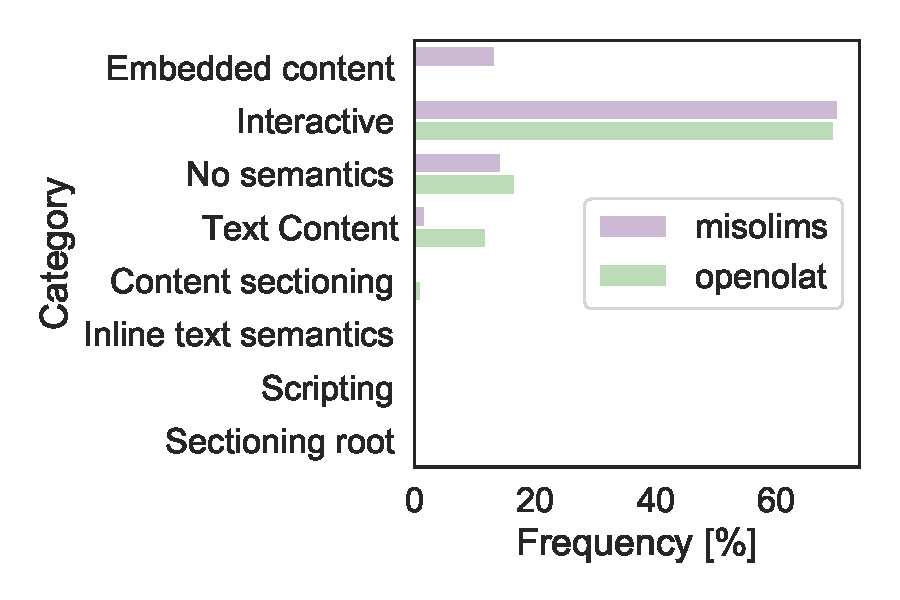
\includegraphics[width=0.7\textwidth]{figures/hpath/category-target-frequency.pdf}\label{fig:hpath-results-frequency-target}}
\subfigure[Present in DOM]{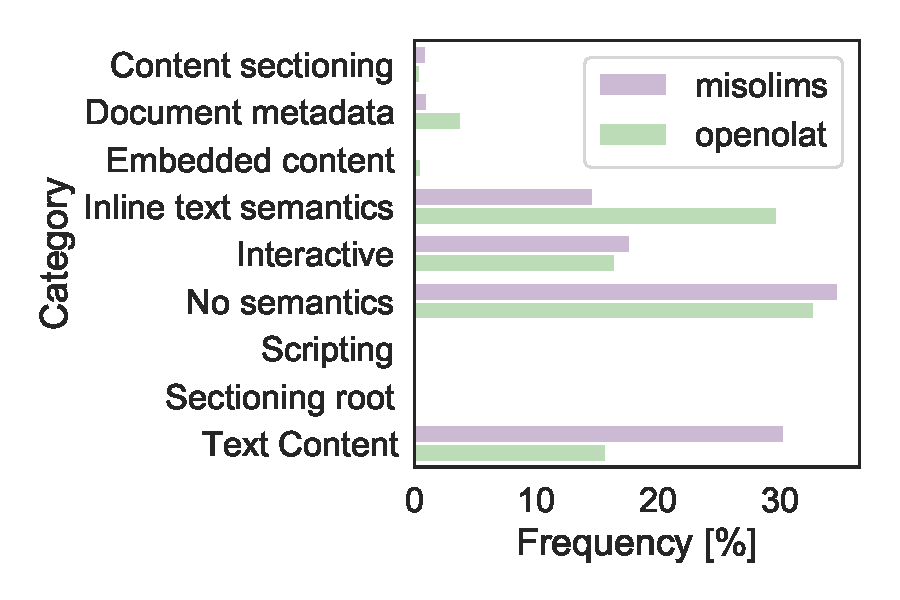
\includegraphics[width=0.7\textwidth]{figures/hpath/category-dom-frequency.pdf}\label{fig:hpath-results-frequency-dom}}
\caption{Percentages of elements (a) targeted by GUI-based tests and (b) present in the DOM for MISO LIMS and OpenOLAT across all versions aggregated by category.}  
\label{fig:hpath-results-frequency}
\end{figure}

In this RQ we evaluate the prevalence of each type of element targeted by GUI-based tests. Indeed, HPath makes strong assumptions about the type of elements being targeted by tests. For instance, elements from the Inline Text Semantics category and elements with no semantic attached ($E_{div}$ and $E_{span}$) that are not rendered cannot be reached by our approach. Furthermore, two (\emph{label} and \emph{text}) out of the four predicates present in the current implementation specifically target elements of the Interactive category. The institution behind these assumptions is that GUI-based tests interact with the application in the same fashion as a user would, through visible GUI components. 

Figure~\ref{fig:hpath-results-frequency} presents the distribution of target elements grouped by their semantic categories. It contrasts the frequency of elements targeted by GUI-based tests (Figure~\ref{fig:hpath-results-frequency-target}) to their overall frequency in the HTML document (Figure~\ref{fig:hpath-results-frequency-dom}). The discrepancy between the two shows that not all elements are of interest to testers. Indeed, the most prevalent categories in the HTML documents are No Semantics with 34.77\% and 32.82\% for MISO LIMS and OpenOLAT respectively, Inline Text Semantics with 29.76\% for OpenOLAT and Text Content with 30.32\% for MISO LIMS. However, Figure~\ref{fig:hpath-results-frequency-target} shows a very different picture, where the overwhelming category is Interactive with 70.27\% and 69.70\% for MISO LIMS and OpenOLAT respectively, confirming our hypothesis.

However, looking at Figure~\ref{fig:hpath-results-frequency-target} we observe a non-negligible amount of elements with no semantics accounting for 14.45\% in MISO LIMS and 16.71\% in OpenOLAT. After reviewing the tests it appears that some assertions and synchronization points target portions of the DOM defined by a $e_{div}$. Therefore, while they do not hold any intrinsic semantic in the HTML standard they do act as an anchor point that can be targeted by test scripts to assess the presence of an underlying group of elements. A more detailed discussion is presented in Section~\ref{sec:hpath-results-rq2} regarding the impact on HPath.

Finally, two categories vary from one project to the other, namely, Embedded content and Text content. The presence of elements from the Embedded content in MISO LIMS (13.41\%) is explained by clickable images under an anchor element, thus behaving like Interactive Elements. As for the elements from Text Content category present in OpenOLAT (11.91\%), they are used when asserting that the SUT is in the expected state, thus, following our hypothesis.

To conclude this research question, we see that GUI-based tests typically target specific portions of the HTML document, namely, Interactive elements and visible components on the page (text and images). HPath, relies on relevant properties to specify these elements and offers good predicates when locating them. However, the proportion of target elements with no HTML semantic is not negligible, which could make HPath enable to locate these elements if they are not rendered on the screen. We investigate this possibility in the next research question. 

\subsection{RQ2: Element Properties Used by Locators}
\label{sec:hpath-results-rq2}

This RQ investigates the relative performance in exploiting properties of target elements in the location path. HPath, absolute XPath and Robula+ formulating different hypotheses on which properties of an element can be used to locate it, we compare the three approaches.

Before being able to analyze which properties of the DOM HPath can leverage, we need to ensure that the target elements are reachable by the technique. Indeed, as shown in Section~\ref{sec:hpath-results-rq1} around 15\% of the target elements might not be rendered on the page. It appears that HPath fails to retrieve the locator in 11.58\% of the cases for MISO LIMS and in 10.48\% for OpenOLAT. These target elements not being rendered on the page, HPath is enabled to retrieve them. When observing the data, we see that assertions and synchronization points can target $e_{div}$ to verify the presence of the underlying group of elements. However, in many cases, other elements could have been selected to yield the same result had the initial test automation engineer relied on HPath. For example, in the project OpenOLAT, a test waits for a calendar widget to be rendered on a page, thus waits for the containing $e_{div}$ identified by its id (fc-view-container). The widget offering a series of named buttons (monat, tag, jhar) the test could rely on those to assess the availability of the widget. In the remaining of the discussion, only elements reachable by HPath are considered.

\begin{figure}
\centering
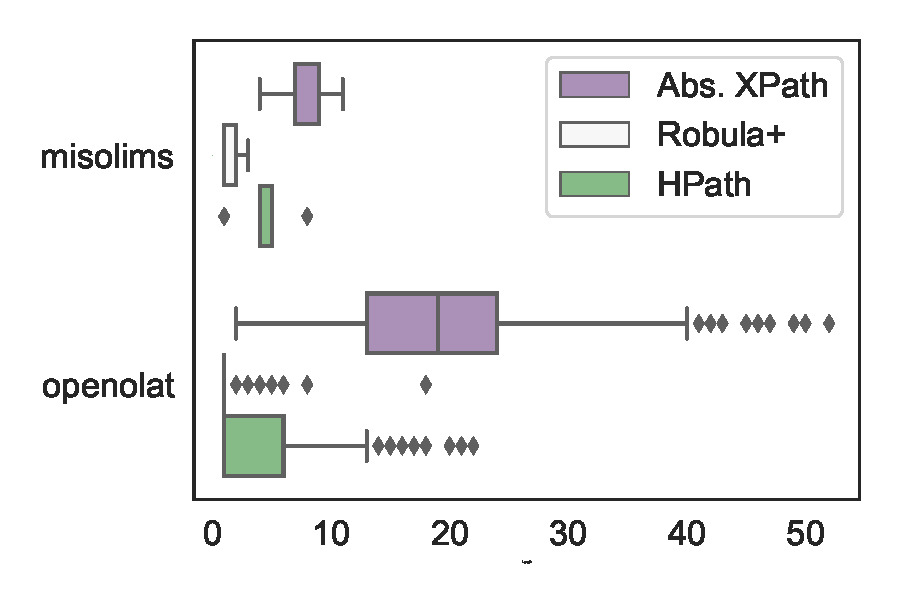
\includegraphics[width=0.6\columnwidth]{figures/hpath/canonical-selector-complexity-dist.pdf}
\caption{Length of absolute XPath, HPath and Robula+ for MISO LIMS and OpenOLAT across all versions.}  
\label{fig:hpath-results-lengths}
\end{figure}

We can now start our discussion on the properties by analyzing how much of the tree hierarchy is leaked when generating the location path. Figure~\ref{fig:hpath-results-lengths} displays the distribution of the length of the locators for the three strategies: absolute XPath, $L_{AXPath}$, Robula+ $L_{Robula+}$, and HPath, $L_{HPath}$. The figure shows a similar trend in both projects where absolute XPath yields the longest location paths with an average length of 8.6 and 18.7, Robula+ the shortest location path, with 1.6 and 1.0 and HPath lies between the two with 4.4 and 3.1, for MISO LIMS and OpenOLAT respectively. The lower performances of absolute XPath are to be expected since if no optimization can be done, both Robula+ and HPath generate a location path that is equal to the absolute XPath. Therefore $L_{HPath} \leq L_{AXPath}$ and $L_{Robula+} \leq L_{AXPath}$.

We compare the different distributions $L_{AXPath}$, $L_{Robula+}$ and $L_{HPath}$ using statistical Wilcoxon signed-rank test\footnote{Shapiro-Wilk test ($\alpha=0.001$) shows the non-normality of the distribution} ($\alpha=0.001$). The goal of this test is to assess whether or not there exists a statistical difference between the pairwise distributions. The results show that there is indeed a difference between all distributions, hence, the different strategies yield locators with different lengths. Then, we compute the pairwise effect size to determine how often lengths from one distribution are greater than in the other. The results show that in all the cases, the size effect is close to 1, \emph{i.e.} all samples from one distribution are greater than in the other, with the exception of $L_{HPath}$ and $L_{Robula+}$ for the OpenOLAT project where the size effect is 0.68. This is due to the fact that in many cases (58.52\% for HPath and 97.72\% for Robula+) both strategies manage to generate a location path of size 1, \emph{i.e.} not leaking hierarchy details of the DOM.

To conclude this discussion on the length of the location paths, we can see that strategies relying on different properties yield locators with different lengths. Relying on element attributes generates the shortest location path in both approaches and HPath exhibits better performances for OpenOLAT than MISO LIMS, even though the tree is deeper (as shown by the length of the absolute XPath). This is a consequence of OpenOLAT using the HTML5 standard, where MISO LIMS implements HTML4, offering more opportunities for HPath to generate good predicates.

\begin{table}
\caption{Properties of the context element leveraged by HPath and Robula+ predicates. \emph{Count} is the number of locators using a property as a predicate and \emph{\%} is the percentage among all the locators collected.}
\label{tab:hpath-results-properties}
\begin{center}
\begin{tabular}{>{\raggedright}m{0.4in}>{\raggedright}m{0.5in}>{\raggedleft}m{0.25in} >{\raggedleft}m{0.2in}>{\raggedleft}m{0.4in} >{\raggedleft}m{0.2in}}
\toprule
\textbf{\scriptsize{Strategy}} & \textbf{\scriptsize{Property}} & \multicolumn{2}{c}{\textbf{\scriptsize{MISO LIMS}}} & \multicolumn{2}{c}{\textbf{\scriptsize{OpenOLAT}}}\tabularnewline
&   & \textbf{\scriptsize{Count}} & \textbf{\scriptsize{\%}} & \textbf{\scriptsize{Count}} & \textbf{\scriptsize{\%}}\tabularnewline
\toprule
\scriptsize{\textit{HPath}} & \scriptsize{\textit{caption}} & \scriptsize{0} & \scriptsize{0.00} & \scriptsize{0} & \scriptsize{0.00}\tabularnewline
& \scriptsize{\textit{figcaption}} & \scriptsize{0} & \scriptsize{0.00} & \scriptsize{0} & \scriptsize{0.00}\tabularnewline
& \scriptsize{\textit{label}} & \scriptsize{0} & \scriptsize{0.00} & \scriptsize{31048} & \scriptsize{16.03}\tabularnewline
& \scriptsize{\textit{legend}} & \scriptsize{0} & \scriptsize{0.00} & \scriptsize{22354} & \scriptsize{11.54}\tabularnewline
& \scriptsize{\textit{text}} & \scriptsize{227} & \scriptsize{1.64} & \scriptsize{93031} & \scriptsize{48.02}\tabularnewline
& \scriptsize{\textit{\textbf{total}}} & \scriptsize{\textbf{227}} & \scriptsize{\textbf{1.64}} & \scriptsize{\textbf{142103}} & \scriptsize{\textbf{73.35}}\tabularnewline
\hline
\scriptsize{\textit{Robula+}} & \scriptsize{\textit{id attr.}} & \scriptsize{5161} & \scriptsize{32.93} & \scriptsize{143334} & \scriptsize{66.23}\tabularnewline
& \scriptsize{\textit{class attr.}} & \scriptsize{412} & \scriptsize{2.63} & \scriptsize{48483} & \scriptsize{22.40}\tabularnewline
& \scriptsize{\textit{name attr.}} & \scriptsize{207} & \scriptsize{1.32} & \scriptsize{150} & \scriptsize{0.07}\tabularnewline
& \scriptsize{\textit{title attr.}} & \scriptsize{0} & \scriptsize{0.00} & \scriptsize{3094} & \scriptsize{1.43}\tabularnewline
& \scriptsize{\textit{text}} & \scriptsize{0} & \scriptsize{0.00} & \scriptsize{17751} & \scriptsize{8.20}\tabularnewline
& \scriptsize{\textit{\textbf{total}}} & \scriptsize{\textbf{5780}} & \scriptsize{\textbf{36.88}} & \scriptsize{\textbf{212558}} & \scriptsize{\textbf{99.80}}\tabularnewline
\bottomrule
\end{tabular}
\end{center}
\end{table}

Therefore, we conduct a fine-grained analysis to understand which properties HPath and Robula+ are able to leverage to compute the location path. Table~\ref{tab:hpath-results-properties} shows which element properties are exploited in the predicates of both approaches. Where HPath relies on properties from the HTML5 semantics, Robula+ exploits mainly attributes of the context element to generate the predicate.

Rows \emph{total} from Table~\ref{tab:hpath-results-properties} indicates how often a strategy is able to compute a predicate. We can see that in the case of OpenOLAT, both strategies often manage to compute predicate (73.35\% for HPath and 99.80\% for Robula+) but a lot less often in the case of MISO LIMS (1.64\% for HPath and 36.88\% for Robula+). Putting the results for MISO LIMS in contrast with the ones presented in Figure~\ref{fig:hpath-results-lengths}, we see that both strategies rely on other mechanisms to reduce the length. HPath relies on the rendering tree to prune $e_{div}$ that are not rendered. On the other hand, Robula+ during each refinement step evaluates the current location path to see if it uniquely identifies the target element. Doing so, it is able to take advantages of the fact that some element types are unique in the document, leading to location path such as "//img" in documents containing a single $e_{img}$ and manages to create a relative path 100\% of the time. However, relying on the uniqueness of an element type in a document can lead to locator breakages during SUT evolution, thus this strategy is not employed by HPath.

%we can see that in the case of MISO LIMS, the algorithm is almost never (1.64\%) capable of using a predicate while in the case of OpenOLAT, it is capable of relying on a predicate more than 70\% of the time. This drastic difference is explained by different factors. First, OpenOLAT uses HTML5 which has a much richer semantic that can be exploited by HPath while MISO LIMS uses the HTML4 standard. Further analysis showed that a lot of the interaction with MISO LIMS element are actually cells located in tables. Unfortunately, HPath does not yet support any predicate that allow to extract semantically element of a table. Finally, even though some semantic elements existed in HTML4, the developers of MISO LIMS do not rely on them and prefer the heavy use of $E_{div}$, lacking semantic. However, as shown in Figure~\ref{fig:automatic_length_distribution}, HPath is able to shorten the expressions by removing the non visible $e_{div}$ from the expression.

The next point of our discussion addresses the type of predicate used by HPath. As expected, in the case of MISO LIMS, all predicates targeting HTML5 semantic elements cannot be leveraged and only the label property is used. In the case of OpenOLAT, two types of predicates are never used: \emph{caption} and \emph{figcaption}. Analyzing the HTML documents, it appears that none of them contain elements $e_{caption}$ or $e_{figcaption}$. The three remaining predicates \emph{label}, \emph{legend} and \emph{text} are all related to forms ($E_{legend}$) and interactive elements ($E_{label}$ and $N_{text}$ child of Interactive element) and can be successfully used by the HPath predicate.

Robula+ on the other hands relies on the attributes of the element to compute the predicate. We see that almost all the elements of OpenOLAT offer at least one attribute that can be used (91.60\%). However, in 8.20\% of the cases, Robula+ relies on the text contained in the element. Note that the text extraction of Robula+ consists in retrieving the content the child $n_{text}$ of the context element where HPath is relying on the process described in Section~\ref{sec:hpath-hpath-text-extraction}.

In conclusion, results show that HPath is able to compute a location path in 90\% of the cases and when HTML5 semantics are available in the HTML document, HPath is able to successfully compute predicates for over 70\% of target elements. In the cases where no HTML5 semantic is available HPath is still able to reduce the length of the location path by relying on the rendering tree it computes. Nevertheless, relying on attributes properties shows better results, but we argue that those properties are less resistant to change in the SUT and investigate it in the next research question.

\subsection{RQ3: Locators Resilience to SUT Evolution}
\label{sec:locator_evolution_analysis_results}

This third research question evaluates the impact of changes in the SUT on DOM-based locators. Relying on the methodology described in Section~\ref{sec:hpath-protocol-breakage-detection} we present in Table~\ref{tab:locator_breakage} the percentage of locators breakage following SUT evolution. 

The results show that the two projects have very different profiles. Indeed, locator breakages depending on the type of the properties evolving in the SUT, they may vary from one development cycle to the next. However, note that the two projects are quite mature with over 15,000 commits in almost 10 years for OpenOLAT and over 4,200 commits in 9 years for MISO LIMS. This explains why no deep structural changes are observed over the periods we analyze as the low breakage count for absolute XPath suggests. Our goal being to spot iso-functional locator breakages, this stability ensures that when a breakage is observed, it is not due to a deep functional evolution of the page.

From Table~\ref{tab:locator_breakage}, for MISO LIMS, Robula+ has the lowest number of breakages (10) and closely followed by HPath (26). Figure~\ref{fig:changes_intersect_misolims} shows the intersection of elements for which the locators break. It shows that absolute XPath is a superset of Robula+ and HPath suggesting that they only break following a change in the DOM hierarchy. Furthermore, there is no overlap between Robula+ and HPath, meaning that relying on different properties make the locators resilient to different types of SUT evolution (supporting the results from Leotta\etal\cite{Leotta2015}).

On the other hand, the OpenOLAT project offers a very different picture. When constructing the HTML document to serve to the client, the backend of OpenOLAT automatically generates id, based on the version of the project, in order to ease communication with the database management system. HPath offers in this case the best resilience to change breaking only 0.49\% of the time. Contrarily, Robula+, relying on element attributes, offers very poor performance breaking in 64.99\% of the cases. Figure~\ref{fig:changes_intersect_misolims} shows that there exists an overlap between the different strategies but that in general they all react differently to changes.

\begin{table}
\caption{Locator breakages due to SUT evolution. \emph{Count} is the number of locators that broke because of a change and \emph{\%} is the percentage among all the pairs collected.}
\label{tab:locator_breakage}
\begin{center}
\begin{tabular}{>{\raggedright}m{0.6in}>{\raggedleft}m{0.4in} >{\raggedleft}m{0.2in}>{\raggedleft}m{0.4in} >{\raggedleft}m{0.2in}}
\toprule
\textbf{\scriptsize{Strategy}} & \multicolumn{2}{c}{\textbf{\scriptsize{MISO LIMS}}} & \multicolumn{2}{c}{\textbf{\scriptsize{OpenOLAT}}}\tabularnewline
    & \textbf{\scriptsize{Count}} & \textbf{\scriptsize{\%}} & \textbf{\scriptsize{Count}} & \textbf{\scriptsize{\%}}\tabularnewline
\toprule
\scriptsize{\textit{Abs. XPath}} & \scriptsize{56} & \scriptsize{2.02} & \scriptsize{174} & \scriptsize{0.63}\tabularnewline
\scriptsize{\textit{Robula+}} & \scriptsize{10} & \scriptsize{0.36} & \scriptsize{17976} & \scriptsize{64.99}\tabularnewline
\scriptsize{\textit{HPath}} & \scriptsize{26} & \scriptsize{0.94} & \scriptsize{135} & \scriptsize{0.49}\tabularnewline
\bottomrule
\end{tabular}
\end{center}
\end{table}

\begin{figure}
\centering
\subfigure[MISO LIMS]{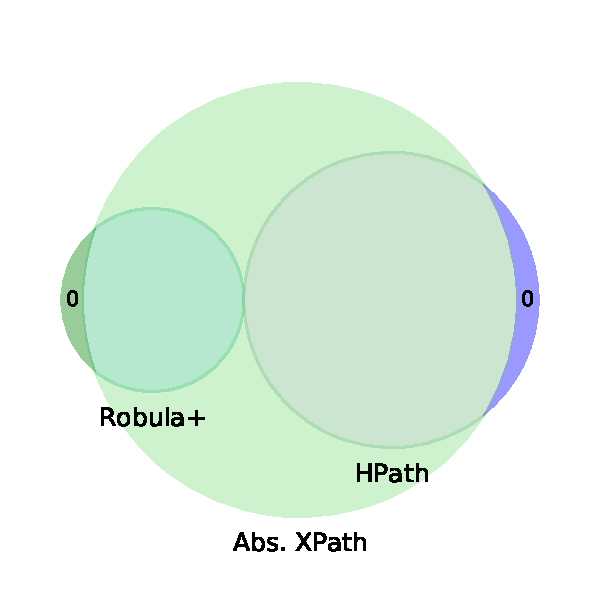
\includegraphics[width=0.7\columnwidth]{figures/hpath/changes-intersect-misolims.pdf}\label{fig:changes_intersect_misolims}}
\subfigure[OpenOLAT]{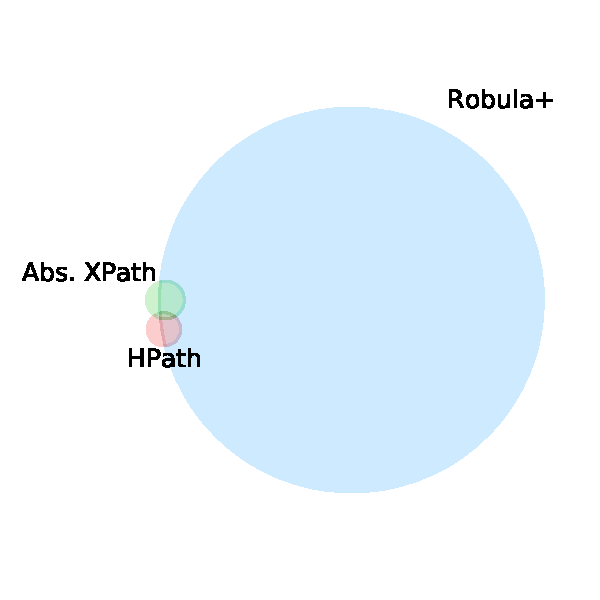
\includegraphics[width=0.7\columnwidth]{figures/hpath/changes-intersect-openolat.pdf}\label{fig:changes_intersect_openolat}}
\caption{Overlap of locators having breakage for Absolute XPath (green), Robula+ (blue) and HPath (red).}  
\label{fig:changes_intersect}
\end{figure}

To better understand which properties of the elements causes the locators to break, Table~\ref{tab:breakage_cause} shows the origin of the failure of the locator. To compute the origin, we compared the breaking location path from  $version_A$ to the passing one computed from $version_B$. The results of the fine-grained difference algorithm between the pair of locators point out the cause of the breakage. 

In the case of MISO LIMS, most of the failures happened in the position predicate, this related to the hierarchy structure of the DOM. Again, in the case of OpenOLAT, the profile is more diverse. Robula+ is not affected by changes in the element types (NameTest) in comparison to the other approaches, but is sensitive to attributes changes, leading to poor resilience to the evolution of the SUT where breakage due to the id contributed to 97.61\% of the breakage. Finally, when HPath is able to compute a predicate, it is resilient and never breaks in our dataset (Row \emph{Any Predicate} from Table~\ref{tab:breakage_cause}).  

\begin{table}[!t]
\caption{Properties causing locator breakages. \emph{Count} is the number of locators breaking because of a property and \emph{\%} is the percentage among all the breaking locators for that strategy.}
\label{tab:breakage_cause}
\begin{center}
\begin{tabular}{>{\raggedright}m{0.4in}>{\raggedright}m{0.8in}>{\raggedleft}m{0.25in} >{\raggedleft}m{0.2in}>{\raggedleft}m{0.4in} >{\raggedleft}m{0.2in}}
\toprule
\textbf{\scriptsize{Strategy}} & \textbf{\scriptsize{Cause}} & \multicolumn{2}{c}{\textbf{\scriptsize{MISO LIMS}}} & \multicolumn{2}{c}{\textbf{\scriptsize{OpenOLAT}}}\tabularnewline
 &   & \textbf{\scriptsize{Count}} & \textbf{\scriptsize{\%}} & \textbf{\scriptsize{Count}} & \textbf{\scriptsize{\%}}\tabularnewline
\toprule
\scriptsize{\textit{Abs. XPath}} & \scriptsize{\textit{NameTest}} & \scriptsize{0} & \scriptsize{0.00} & \scriptsize{60} & \scriptsize{34.48}\tabularnewline
 & \scriptsize{\textit{Predicate position}} & \scriptsize{56} & \scriptsize{100.00} & \scriptsize{114} & \scriptsize{65.52}\tabularnewline
 \hline
\scriptsize{\textit{Robula+}} & \scriptsize{\textit{NameTest}} & \scriptsize{0} & \scriptsize{0} & \scriptsize{11} & \scriptsize{0.06}\tabularnewline
 & \scriptsize{\textit{Predicate position}} & \scriptsize{10} & \scriptsize{100.00} & \scriptsize{2} & \scriptsize{0.01}\tabularnewline
 & \scriptsize{\textit{Predicate id attr.}} & \scriptsize{0} & \scriptsize{0.00} & \scriptsize{17578} & \scriptsize{97.79}\tabularnewline
 & \scriptsize{\textit{Predicate class attr.}} & \scriptsize{0} & \scriptsize{0.00} & \scriptsize{11} & \scriptsize{0.06}\tabularnewline
 & \scriptsize{\textit{Predicate title attr.}} & \scriptsize{0} & \scriptsize{0.00} & \scriptsize{77} & \scriptsize{0.43}\tabularnewline
 & \scriptsize{\textit{Predicate text content}} & \scriptsize{0} & \scriptsize{0.00} & \scriptsize{281} & \scriptsize{1.56}\tabularnewline
 \hline
\scriptsize{\textit{HPath}} & \scriptsize{\textit{NameTest}} & \scriptsize{0} & \scriptsize{0.00} & \scriptsize{119} & \scriptsize{88.14}\tabularnewline
 & \scriptsize{\textit{Predicate position}} & \scriptsize{26} & \scriptsize{100.00} & \scriptsize{16} & \scriptsize{11.85}\tabularnewline
 & \scriptsize{\textit{Any Predicate}} & \scriptsize{0} & \scriptsize{0.00} & \scriptsize{0} & \scriptsize{0.00}\tabularnewline
\bottomrule
\end{tabular}
\end{center}
\vspace{-2em}
\end{table}

In conclusion, when HPath can generate predicates they lead to robust and flexible locators. However, it can be hard for the approach to extract the necessary properties as shown in section~\ref{sec:locator_evolution_analysis_results}. Therefore, while the results are promising, more research needs to be conducted to better exploit the rendering properties present in the HTML5 semantics. Furthermore, better reliance on the standard by developers would improve the performances of tool relying on the semantic of the language.

\section{Threats to Validity}

The goal of HPath is to ease interaction with visible components of a web page through automated GUI-based test scripts. Hence, HPath relies heavily on rendered properties to characterize target elements and only rendered elements are reachable by the approach. Nonetheless, section~\ref{sec:hpath-results-rq1} shows that elements that are not displayed (\emph{e.g.} containing $e_{div}$ of a modal window) can be targeted by the testers. This limitation shows that the goal of HPath is not to replace the currently available strategies but to offer better tool for automation engineers and answer their specific use case.

Furthermore, relying on the HTML standard, some elements provide information about the structure of the document but are not displayed. For instance, many elements from the Content Section category (see Table~\ref{tab:hpath-introduction-html5}) like $E_{article}$ or $E_{section}$ are not rendered but define the flow of the document. Though, because these elements do provide context and semantic, the current implementation of HPath keeps them to offer expressive locators that are easier to understand and potentially adapt.

Finally, conducting our case study on two projects, the conclusions we draw may not hold true for other projects. This constitutes a major threat to the external validity for the generalization of our results outside the context of this study. However, the two projects have very different profiles, thus making the study covering boundary cases among the full range of possible projects. To further alleviate this limitation, we provide a full replication package\footnote{Available at \emph{link not available for double blind process}} to encourage other teams to replicate and extend our results.

\section{Conclusions}

We presented HPath, a novel DOM-based locator strategy to generate location paths more flexible for web testing. We have compared its potential to extract properties from the HTML document and its fragility under SUT evolution against state-of-the-art algorithm Robula+. Our results show that when HTML5 semantics are present, HPath can exploit rendered properties of web elements to generate expressive locators in 73.35\% reducing locator breakages from 64.99\% when relying on attribute properties to 0.49\% with rendered properties. However, in its current form, it is not always able to extract rendered properties to create good location paths and  leaks the hierarchical structure of the DOM for 41.48\% of the elements.

Thus, in our short-term future work, we plan to (1) experiment HPath with more application by extending the support of \mercator\ to other languages implementing the Selenium API, (2) explore more opportunities to generate good predicates relying on heuristics present in the HTML documents such as section titles, overlays, etc. (3) explore ways to generate a rendering tree closer to the GUI components displayed on the screen to better abstract away structural details of the DOM.